\documentclass[11pt]{article}

\usepackage[a4paper,margin=0.85in]{geometry}
\usepackage{booktabs}
\usepackage{array}
\usepackage{longtable}
\usepackage{xcolor}
\usepackage{hyperref}
\usepackage{enumitem}
\usepackage{tikz}
\usetikzlibrary{arrows.meta,positioning,shapes.geometric}

\hypersetup{
  colorlinks=true,
  linkcolor=black,
  urlcolor=blue
}
\setlist[itemize]{leftmargin=1.2em}
\setlist[enumerate]{leftmargin=1.4em}

\definecolor{accent}{HTML}{0D6F58}
\definecolor{soft}{HTML}{F3F7F4}
\definecolor{warn}{HTML}{8A5A00}

\newcommand{\product}{Small-Cap Radar}
\newcommand{\studentid}{b11902138}
\newcommand{\githuburl}{\url{https://github.com/kopojen/new-token-intelligence}}
\newcommand{\livedemo}{\url{https://new-token-intelligence.vercel.app}}

\title{\vspace{-2em}\textbf{\product}\\
\large Designing a System That Monetizes Data}
\author{Student ID: \studentid}
\date{Big Data Systems, Spring 2026}

\begin{document}
\maketitle

\begin{center}
\begin{tabular}{r p{0.62\textwidth}}
\textbf{GitHub Repository:} & \githuburl \\
\textbf{Live Demo:} & \livedemo \\
\textbf{PDF Filename:} & \texttt{b11902138.pdf} \\
\end{tabular}
\end{center}

\vspace{0.5em}
\noindent\textbf{Executive Summary.}
\product{} is a market-intelligence data product for active retail crypto traders who monitor small-cap and high-beta tokens. It combines exchange/event information with Binance market data and turns scattered public data into a dashboard of movers, volume expansion, liquidity, spread, and event context. The product is decision support, not a trading bot or financial advice. Its monetized value is saved monitoring time.

\section{Target Customer}

The target customer is an active retail crypto trader or a small trading community that frequently monitors small-cap tokens, meme coins, new listings, and short-term market movers. This segment is a practical wedge because the workflow is repeated, time-sensitive, and fragmented. Today, these users manually check:
\begin{itemize}
  \item exchange announcement pages from Binance, OKX, KuCoin, and similar sources;
  \item price and market-data pages such as CoinGecko, TradingView, and Binance;
  \item Telegram, Discord, X, and other community channels;
  \item order-book spread, liquidity depth, and recent volume before deciding whether a token deserves attention.
\end{itemize}

The customer job-to-be-done is: \emph{help me quickly see which small-cap or fast-moving tokens deserve deeper manual research before I waste time checking every chart and announcement page myself}. Casual long-term investors are not the initial target because they do not perform this monitoring workflow often enough to justify a paid product.

\section{Evidence of Demand and Customer Investment}

\subsection{Data-Acquisition Process for Demand Evidence}

The demand evidence was collected to answer one question: do active crypto traders already have a repeated monitoring problem that a small-cap token dashboard could reduce? The data-acquisition process uses four sources of evidence.

\textbf{Manual workflow observation.}
I decomposed the existing manual workflow: checking announcements, scanning top gainers, opening short-term charts, validating volume, checking liquidity, and reading community discussion. This takes about 25 to 50 minutes per session, or roughly 3 to 6 hours per week if repeated daily.

\textbf{User validation.}
The planned user survey asks whether respondents trade crypto, monitor new or small-cap tokens, which sources they check, how much time they spend, what pain point is largest, and what time/effort/money they would invest in a dashboard. Before final submission, the pilot rows should be replaced with 5 to 10 real responses.

\textbf{Public data acquisition.}
The prototype structures public event and market data. Event evidence comes from exchange announcement sources and a reproducible local event feed. Market evidence comes from Binance Spot public data: price, movement, volume, spread, and depth. The export command below records announcement evidence in a structured CSV:
\begin{verbatim}
PYTHONPATH=src python3 scripts/export_announcement_evidence.py \
  --out data/demand_evidence/announcement_evidence.csv
\end{verbatim}
The purpose is not to prove that one token is profitable. It shows that relevant token information is scattered across public sources and can be converted into structured monitoring data.

\textbf{Competitor and substitute analysis.}
Substitutes such as CoinGecko, TradingView, alert tools, Telegram channels, and paid crypto analytics products show that users already spend time and sometimes money to obtain faster market information. The opportunity is a narrower workflow: small-cap movers with liquidity and volume context.

\subsection{Customer Investment: Time, Effort, and Money}

The assignment asks how much time, effort, or money the customer would invest. For this product:
\begin{itemize}
  \item \textbf{Time:} users should understand the dashboard within 5 to 10 minutes. Setup should take under 15 minutes for an individual and under one hour for a small group with custom filters.
  \item \textbf{Effort:} users may configure exchanges, volume bands, and alert thresholds, but should not need complex trading-bot setup.
  \item \textbf{Money:} pricing is based on saved monitoring time and comparable data tools.
\end{itemize}

The proposed pricing model is:
\begin{itemize}
  \item Free tier: delayed daily movers and liquidity summary.
  \item Basic tier: USD 9--19 per month for live dashboard access.
  \item Pro tier: USD 49 per month for custom filters, CSV/API export, and small-community watchlists.
\end{itemize}

If the dashboard saves 3 hours per week and the user's monitoring time is worth USD 10 per hour, the avoided attention cost is about USD 120 per month. A USD 9--19 subscription is therefore a small fraction of the saved monitoring effort. The exact price should still be validated with real responses.

\section{Technical System Design}

\subsection{Data Sources}

The prototype ingests or structures:
\begin{itemize}
  \item Binance Spot public REST market data: price, 24h volume, spread, depth, and recent movement for the live dashboard.
  \item Binance Alpha public token list and exchange announcement sources.
  \item OKX and KuCoin announcement pages.
  \item Local reproducible event feed at \texttt{data/local\_event\_feed.json}.
  \item Local reproducible market snapshot at \texttt{data/sample\_market\_snapshot.json}.
\end{itemize}

The deployed Vercel demo runs a live Binance Spot public market scan and applies the small-cap filter at request time. The local fallback demo uses fixed real Binance spot pairs such as \texttt{MEMEUSDT}, \texttt{ORDIUSDT}, \texttt{WIFUSDT}, \texttt{BONKUSDT}, \texttt{PEPEUSDT}, and \texttt{FLOKIUSDT} only to keep the course demo reproducible when network access is unavailable.

\subsection{Processing and Storage}

For a course-scale prototype, local JSON fixtures and direct HTTP ingestion are appropriate because they keep the system reproducible. The pipeline performs:
\begin{enumerate}
  \item event ingestion and symbol extraction;
  \item small-cap universe filtering by excluding major base assets and applying a configurable 24h quote-volume band;
  \item market feature extraction for price, returns, volume expansion, spread, depth, and trade-count proxies;
  \item dashboard row construction for movers, market snapshots, market notes, and event notes;
  \item delivery through a live Vercel dashboard, CLI output, and CSV evidence exports.
\end{enumerate}

The small-cap proxy excludes major base assets and applies a configurable 24h quote-volume band. This is not a perfect market-cap measurement, but it is transparent and reproducible without adding a separate paid market-cap data dependency.

\subsection{Delivery}

The customer consumes the product through a web dashboard. The current dashboard has these sections:
\begin{itemize}
  \item Watchlist: fast movers ranked by 24h movement and volume expansion.
  \item Current Focus and Liquidity Lens: the strongest current mover plus spread/depth context.
  \item Momentum Board: top 24h movers with price, 1h movement, 15m movement, volume spike, and 24h volume.
  \item Market Snapshot: comparable raw indicators across tracked pairs.
  \item Market Notes and Event Notes: liquidity, spread, volume, and event context.
\end{itemize}

The deployed demo is available at \url{https://new-token-intelligence.vercel.app}.
For reproducible fallback testing, the same dashboard can also be run locally from the repository.

\subsection{Architecture Diagram}

\begin{center}
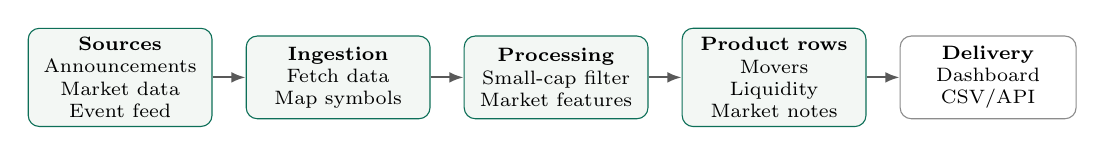
\begin{tikzpicture}[
  node distance=0.42cm,
  box/.style={rectangle, rounded corners, draw=accent, fill=soft, align=center, text width=2.1cm, minimum height=1.05cm, font=\scriptsize},
  outbox/.style={rectangle, rounded corners, draw=black!45, fill=white, align=center, text width=2.0cm, minimum height=1.05cm, font=\scriptsize},
  arrow/.style={-{Latex[length=1.8mm]}, thick, draw=black!65}
]
\node[box] (sources) {\textbf{Sources}\\Announcements\\Market data\\Event feed};
\node[box, right=of sources] (ingest) {\textbf{Ingestion}\\Fetch data\\Map symbols};
\node[box, right=of ingest] (process) {\textbf{Processing}\\Small-cap filter\\Market features};
\node[box, right=of process] (dataset) {\textbf{Product rows}\\Movers\\Liquidity\\Market notes};
\node[outbox, right=of dataset] (deliver) {\textbf{Delivery}\\Dashboard\\CSV/API};

\draw[arrow] (sources) -- (ingest);
\draw[arrow] (ingest) -- (process);
\draw[arrow] (process) -- (dataset);
\draw[arrow] (dataset) -- (deliver);
\end{tikzpicture}
\end{center}

\subsection{Scalability and Cost}

At 10x scale, the main bottleneck is source rate limiting and repeated market-data fetches. The system would need scheduled ingestion, caching, and backoff policies. At 100x scale, it would need a persistent feature store, queue-based processing, and possibly paid data licenses.

\section{Business Model}

The product monetizes processed data rather than raw data. Raw market and announcement data are public, but they are scattered, noisy, and time-sensitive. The dashboard creates value by cleaning, joining, filtering, and presenting those sources in a faster monitoring workflow.

Revenue streams:
\begin{itemize}
  \item subscription for individual active traders;
  \item higher-price plan for small trading communities;
  \item future CSV/API export for users who want to integrate market rows into their own workflow.
\end{itemize}

The main cost drivers are data-source reliability, server costs for frequent refreshes, maintenance of feature rules, and possible paid data licenses if the product grows.

\section{Go-to-Market Difficulties}

This section is included for the bonus component.

The largest challenge is trust: crypto traders may not trust a new dashboard unless fields, sources, and limitations are transparent. The second challenge is false positives because small-cap markets are noisy and volatile. The third challenge is competition from CoinGecko, TradingView, Telegram channels, and paid analytics tools. The fourth challenge is data access: public pages and APIs may change, rate-limit requests, or restrict automated access. Finally, casual users may not pay, so the business must focus on active users who monitor markets often enough that saved time has real value.

\section{Ethics and Legal Considerations}

The dashboard is an educational market-intelligence prototype. It should not be marketed as financial advice or as a promise of profit. It should avoid collecting private user trading data unless there is clear consent and a privacy policy. Data collection should respect source terms of service, robots.txt, rate limits, copyright, and applicable privacy regulations.

\section{Conclusion}

\product{} demonstrates how public market and announcement data can be refined into a monetizable data product. The system collects raw event and market data, transforms it into a monitoring dashboard, and supports a subscription model for active users who value saved monitoring time.

\end{document}
